\renewcommand{\thefigure}{\Asbuk{section}.\arabic{figure}}
\renewcommand{\thetable}{\Asbuk{section}.\arabic{table}}
\renewcommand{\thelstlisting}{\Asbuk{section}.\arabic{lstlisting}}

% \newgeometry{left=1cm,right=1cm,top=1cm,bottom=1cm}
\begin{landscape}
\section*{
  ПРИЛОЖЕНИЕ A \\ 
  (обязательное) \\ 
  Стандарт-план работы участка
}
\addcontentsline{toc}{section}{
  Приложение А (обязательное) Стандарт-план работы участка
}
\label{sec:appendix_a}

\pagestyle{fancy}
\fancyhf{}  % clear all header and footer fields
\fancyfoot[R]{\thepage}
\renewcommand{\headrulewidth}{0pt}
\renewcommand{\footrulewidth}{0pt}

\setlength{\headheight}{10mm}
\setlength{\headsep}{\baselineskip}
\chead{Продолжение приложения \Asbuk{section}}

\thispagestyle{plain}

\setcounter{section}{1}
\setcounter{figure}{0}
\setcounter{table}{0}
\setcounter{lstlisting}{0}

\begin{table} [h!]
  {\scriptsize
    \begin{tabular}{
      | p{2.2cm} | c | c | c | c | c | c | c | c | c 
      | m{1cm} m{1cm} m{1cm} m{1cm} m{1cm} m{1cm} m{1cm} m{1cm} 
      | c |
      }
      \hline
     \multirow{2}{*}{
       \parbox{2.2cm}{
         \vspace{8mm}
         \centering
         Наименование \\ операции
       }
     }
   & \multirow{2}{*}{
       \rotatebox[origin=c]{90}{
         \parbox{2.2cm}{
            Норма времени с \\
            учетом коэф. \\
            выполнения норм \\ 
            (\( t_{\text{шт}}\)), мин
         }
       }
     }
   & \multirow{2}{*}{
       \rotatebox[origin=c]{90}{
         \parbox{2.2cm}{
           Такт потока (\( r_{\text{пр}} \)), \\ мин/шт.
         }
       }
     }
   & \multicolumn{2}{c|}{\parbox{1cm}{\centering Кол-во \\ рабочих \\ мест}}
   & \multirow{2}{*}{
       \rotatebox[origin=c]{90}{
          \parbox{2.2cm}{ \textnumero \hspace{0.5mm} рабочих мест}
       }
     }
   & \multicolumn{2}{c|}{\parbox{1cm}{\centering Загрузка \\ рабочих \\ мест}}
   & \multirow{2}{*}{
       \rotatebox[origin=c]{90}{
         \parbox{2.2cm}{
           Количество \\ рабочих, чел
         }
       }
     }
   & \multirow{2}{*}{
       \rotatebox[origin=c]{90}{
         \parbox{2.2cm}{
            Порядок обслуж. \\ рабочих мест
         }
       }
     }
   & \multicolumn{8}{c|}{
       \parbox{10cm}{
         \centering
         \smallskip
         График работы оборудования и перехода рабочих с одного рабочего
         места на другое за период оборота линии, равный одной смене (480 мин),
         и движение обороных заделов
         \smallskip
       }  
     }
   & \multirow{2}{*}{
       \rotatebox[origin=c]{90}{
         \parbox{2.2cm}{
           Программа~выпуска \\
           дет. за \( F_{\text{см}} = \) \\ \( T_o = 480 \: \text{мин} \)
         }
       }
     } \\ \cline{4-5}\cline{7-8}\cline{11-18}
   & & 
   & \rotatebox[origin=c]{90}{
         \parbox{1.3cm}{
           расчетное \\ (\( C_{\text{р}} \)) 
         }
       }
   & \rotatebox[origin=c]{90}{
         \parbox{1.3cm}{
           принятое \\ (\( C_{\text{пр}} \)) 
         }
       }
   & 
   & \rotatebox[origin=c]{90}{
         \parbox{1.3cm}{
           в \%
         }
       }
   & \rotatebox[origin=c]{90}{
         \parbox{1.3cm}{
           в мин
         }
       }
   & &
   & \multicolumn{8}{c|}{
       \multirow{14}{*}{
         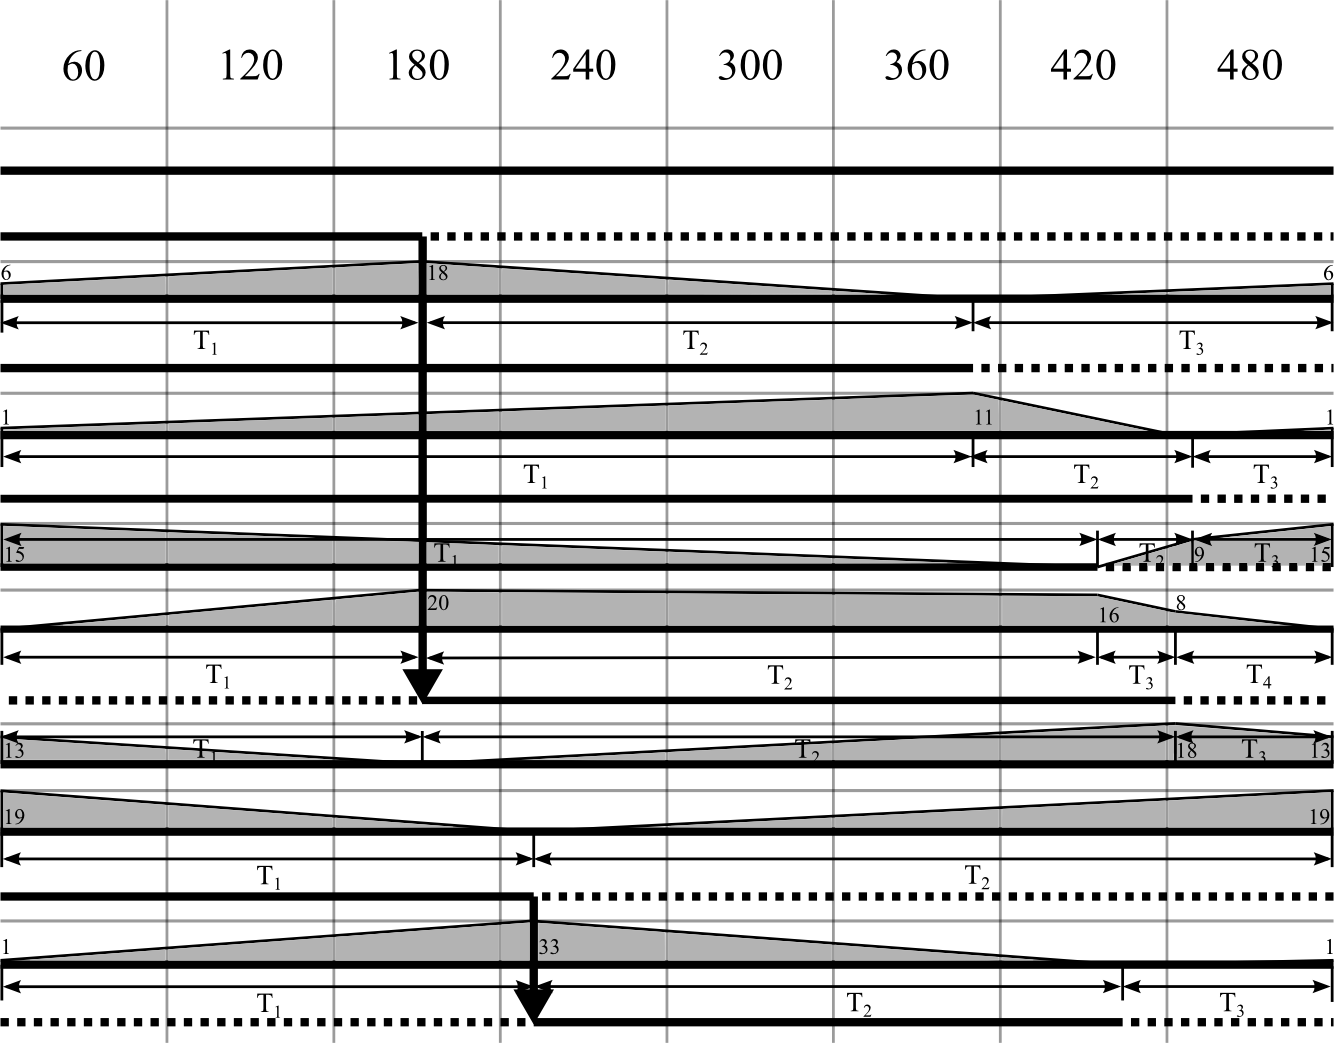
\includegraphics[width=10.7cm]{pic/splan}
       }
     }
   & \\ \cline{1-10}\cline{19-19}

   \multirow{2}{*}{1. Фрезерная} 
   & \multirow{2}{*}{5{,}82} & \multirow{2}{*}{4{,}42}
   & \multirow{2}{*}{1{,}32} & \multirow{2}{*}{2}
   & 1 
   & 100 & 480
   & \multirow{2}{*}{2}
   & 1
   & & & & & & & &
   & 83 \\

   & & & 
   & 
   & 2 
   & 32 & 152
   & 
   & 2 + v
   & & & & & & & &
   & 26 \\ \cline{1-10}\cline{19-19}

   \multirow{2}{*}{2. Шлифовальная} 
   & \multirow{2}{*}{7{,}45} & \multirow{2}{*}{4{,}42}
   & \multirow{2}{*}{1{,}69} & \multirow{2}{*}{2}
   & 3 
   & 100 & 480
   & \multirow{2}{*}{2}
   & 3
   & & & & & & & &
   & 64 \\

   & & & 
   & 
   & 4 
   & 69 & 330
   & 
   & 4 + v
   & & & & & & & &
   & 44 \\ \cline{1-10}\cline{19-19}

   \multirow{2}{*}{3. Слесарная} 
   & \multirow{2}{*}{8{,}36} & \multirow{2}{*}{4{,}42}
   & \multirow{2}{*}{1{,}89} & \multirow{2}{*}{2}
   & 5 
   & 100 & 480
   & \multirow{2}{*}{2}
   & 5
   & & & & & & & &
   & 57 \\

   & & & 
   & 
   & 6 
   & 89 & 429
   & 
   & 6 + v
   & & & & & & & &
   & 51 \\ \cline{1-10}\cline{19-19}

   4. Токарная
   & 3{,}64 & 4{,}42
   & 0{,}82 & 1
   & 7 
   & 82 & 395
   & 1
   & 7
   & & & & & & & &
   & 109 \\ \cline{1-10}\cline{19-19}

   \multirow{2}{*}{5. Фрезерная} 
   & \multirow{2}{*}{6{,}91} & \multirow{2}{*}{4{,}42}
   & \multirow{2}{*}{1{,}56} & \multirow{2}{*}{2}
   & 8 
   & 100 & 480
   & \multirow{2}{*}{2}
   & 8
   & & & & & & & &
   & 69 \\

   & & & 
   & 
   & 9 
   & 56 & 271
   & 
   & 9 + v
   & & & & & & & &
   & 39 \\ \cline{1-10}\cline{19-19}

   6. Слесарная
   & 4{,}55 & 4{,}42
   & 1{,}03 & 1
   & 10 
   & 100 & 480
   & 1
   & 10
   & & & & & & & &
   & 109 \\ \cline{1-10}\cline{19-19}

   \multirow{2}{*}{7. Сверлильная} 
   & \multirow{2}{*}{6{,}18} & \multirow{2}{*}{4{,}42}
   & \multirow{2}{*}{1{,}4} & \multirow{2}{*}{2}
   & 11 
   & 100 & 480
   & \multirow{2}{*}{2}
   & 11
   & & & & & & & &
   & 78 \\

   & & & 
   & 
   & 12 
   & 40 & 192
   & 
   & 12 + v
   & & & & & & & &
   & 31 \\ \cline{1-10}\cline{19-19}

   \multirow{2}{*}{8. Токарная} 
   & \multirow{2}{*}{6{,}36} & \multirow{2}{*}{4{,}42}
   & \multirow{2}{*}{1{,}44} & \multirow{2}{*}{2}
   & 13 
   & 100 & 480
   & \multirow{2}{*}{2}
   & 13
   & & & & & & & &
   & 75 \\

   & & & 
   & 
   & 14
   & 44 & 212
   & 
   & 14 + v
   & & & & & & & &
   & 33 \\ \cline{1-10}\cline{19-19}

   Итого
   & 49{,}27 & 4{,}42
   & 11{,}16 & 14
   & 14 
   & 79 & 
   & 12
   & 
   & & & & & & & &
   & \\ \hline

    \end{tabular}
  }
\end{table}


\end{landscape}
% \restoregeometry
